\section{Experimentación}
\subsection{Mediciones y metodología de experimentación}

Para las mediciones de tiempo se tomó como base la experimentación propuesta
por la cátedra.
% Instancias:
Fueron realizadas mediciones de tiempo para la función \texttt{mstParalelo}
tomando distintas instancias de árboles, grafos ralos y completos, variando la
cantidad de nodos y cantidad de \textit{threads}.
% Repeticiones:
% se repitió 5 veces el llamado a `-e`. Dicho procedimiento usa un for
% i=0,...,9 para correrlo 10 veces obteniendo un total de 50 corridas. El
% procedimiento para correr la experimentación da 1800 filas, nuestro CSV tiene
% 9000 filas.
Debido a la naturaleza no-deterministica de la programación concurrente, se
tomaron 50 corridas para cada instancia (tipo de grafo, cantidad de nodos y
cantidad de \textit{threads}) del problema. En las
figuras~\ref{fig:arboles},~\ref{fig:ralos} y~\ref{fig:completos} se traza el
promedio y se muestra en sombreado el desvío estándar.

% CPU:
Los experimentos fueron medidos en un procesador \texttt{Intel (R) Core (TM) i5
3230M CPU @ 2.60GHz} de 2 \textit{cores} físicos y 4 \textit{cores} lógicos,
con 3072 KB de cache. En una computadora con 8 GB de memoria principal.

\subsection{Resultados}

Se pudo observar que para todos los casos el tiempo de ejecución crece con el
tamaño de la instancia, tanto si su incremento es en cantidad de nodos o en
cantidad de ejes.
% Performance variando #threads
Para todas las instancias obtuvimos una mejor
\textit{performance} al ejecutar de forma secuencial, que al ejecutar más de un
\textit{thread} de forma
concurrente.
% Mas de 4 concurrente:
Puede verse que la degradación de la \textit{performance} se acentúa para las
mediciones de 8, 16 y 32 \textit{threads}, cantidad que supera la cantidad de
\textit{cores} lógicos del CPU donde fueron realizadas las mediciones.

\begin{figure}[h]
\caption{Mediciones para árboles.}
\centering
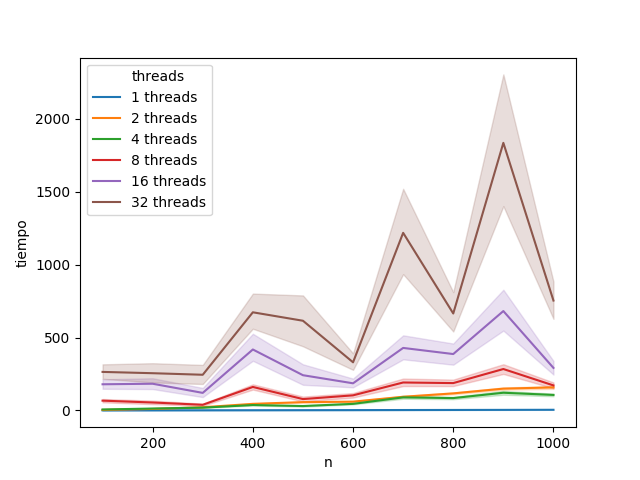
\includegraphics[width=0.5\textwidth]{imagenes/arbol.png} \\%
\label{fig:arboles}
\end{figure}

\begin{figure}[h]
\caption{Mediciones para grafos ralos.}
\centering
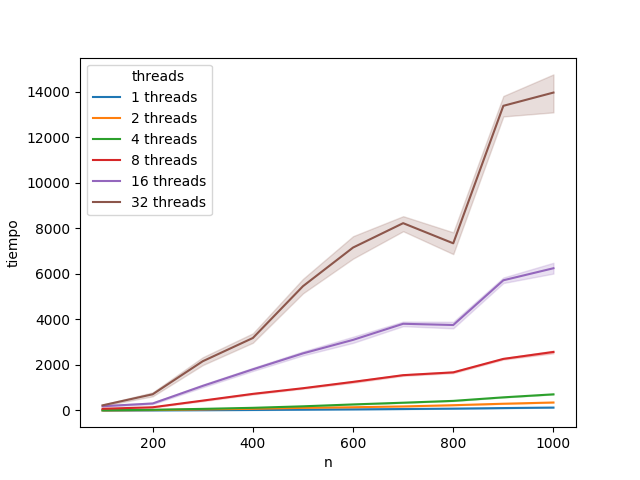
\includegraphics[width=0.5\textwidth]{imagenes/ralo.png} \\%
\label{fig:ralos}
\end{figure}

\begin{figure}[h]
\caption{Mediciones para grafos completos.}
\centering
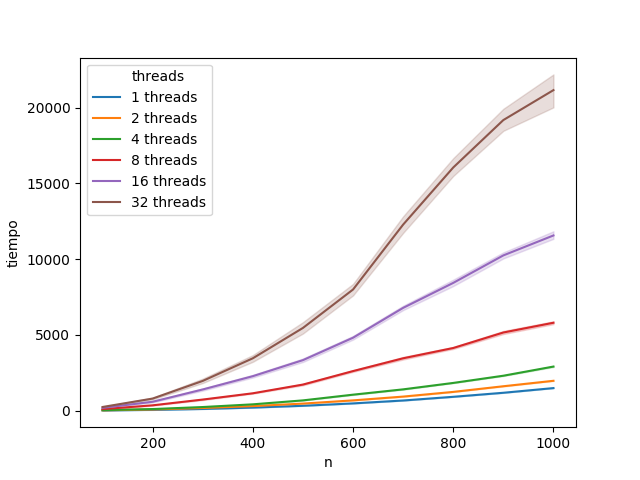
\includegraphics[width=0.5\textwidth]{imagenes/completo.png} \\%
\label{fig:completos}
\end{figure}

%%%%

% Acá hablo de los casos para 1,2,4 threads:
En las figuras~\ref{fig:arboles124}--\ref{fig:completos124} se muestra en
detalle el comportamiento de nuestra implementación del algoritmo para 1, 2 y 4
\textit{threads}. Puede verse que el algoritmo tiene mejor rendimiento de forma
secuencial. Para el caso de los árboles, utilizar 4 threads arrojó
mejores resultados que 2, aunque esta diferencia no es significativa.

\begin{figure}[h]
\caption{Mediciones para árboles con hasta 4 \textit{threads}.}
\centering
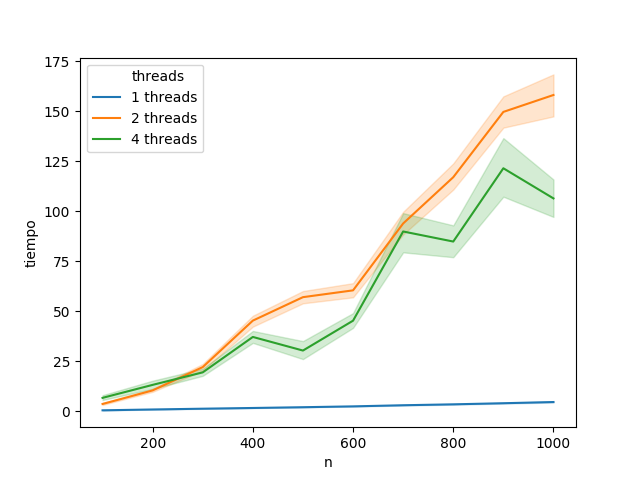
\includegraphics[width=0.5\textwidth]{imagenes/arbol-124.png} \\%
\label{fig:arboles124}
\end{figure}

\begin{figure}[h]
\caption{Mediciones para grafos ralos con hasta 4 \textit{threads}.}
\centering
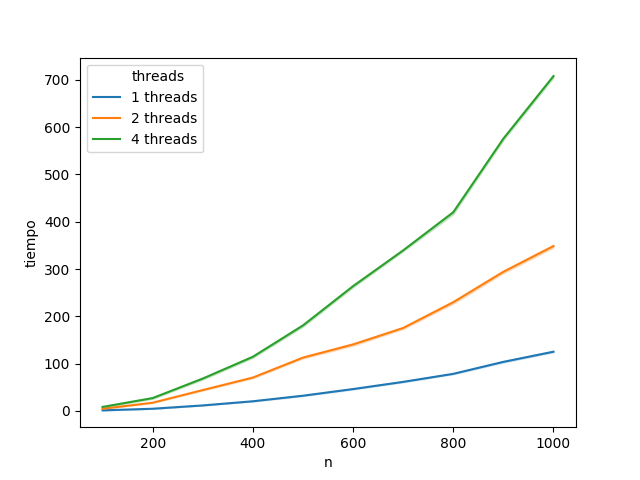
\includegraphics[width=0.5\textwidth]{imagenes/ralo-124.png} \\%
\label{fig:ralos124}
\end{figure}

\begin{figure}[h]
\caption{Mediciones para grafos completos con hasta 4 \textit{threads}.}
\centering
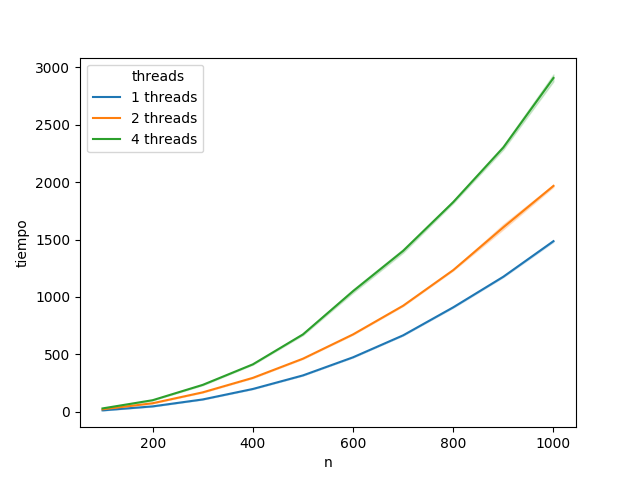
\includegraphics[width=0.5\textwidth]{imagenes/completo-124.png} \\%
\label{fig:completos124}
\end{figure}

La pérdida de rendimiento puede deberse a una mala elección o implementación
del algoritmo y las estructuras que le dan soporte. Al incrementar la 
cantidad de \textit{threads} se incrementa el tiempo en el que los mismos se
 encuentran intentando fusionarse. Las fusiones en sí involucran copiar los 
 datos de un thread al otro y reiniciar a uno de ellos. Todas estas son tareas 
 que el algoritmo secuencial no tiene que hacer. Por otro lado, la penalización
  de los cambios de contexto, inexistente en el caso secuencial, es cada vez 
  mayor a medida que crece la cantidad de threads.
  Otra diferencia entre la versión secuencial y la paralela, es que la última 
  también tiene el overhead de crear, inicializar, detener y sincronizar los 
  hilos. Si estos hilos hacen poco trabajo en relación al overhead que 
  requieren es esperable que haya una pérdida de rendimiento.
% FIXME tirar más hipotesis.
